\documentclass[12pt]{book}

\usepackage{amsmath, amssymb}
\usepackage{tikz} 
\usetikzlibrary{shapes}
\usetikzlibrary{arrows}
\usetikzlibrary{positioning}
\usetikzlibrary{patterns}
\usetikzlibrary{calc}

\usepackage{hyperref}
\hypersetup{
    colorlinks=true, %set true if you want colored links
    linktoc=all,     %set to all if you want both sections and subsections linked
    linkcolor=black,  %choose some color if you want links to stand out
}

\usepackage[margin=1.4in,footskip=.25in]{geometry}


\tikzstyle{input}=[
        draw,
        trapezium,
        trapezium left angle=60,
        trapezium right angle=120,
        inner sep=10pt,
        fill=white!25
]
\tikzstyle{output}=[
        draw,
        trapezium,
        trapezium left angle=60,
        trapezium right angle=120,
        inner sep=10pt,
        fill=white!25
]
\tikzstyle{debutfin}=[ellipse,draw,text=black,inner sep=10pt]
\tikzstyle{instruct}=[rectangle,draw,fill=white!50,inner sep=10pt]
\tikzstyle{test}=[diamond, aspect=1,thick,
draw=black,fill=white!50,text=black]
\tikzstyle{es}=[rectangle,draw,rounded corners=4pt,fill=white!25,inner sep=10pt]
%styledesflèches
\tikzstyle{suite}=[->,>=stealth,thick,rounded corners=4pt]
%placementdesnœuds

\usepackage{xepersian}
\settextfont[Scale=1]{Vazir}

\renewcommand{\baselinestretch}{1.3} 

\begin{document}

\tableofcontents

\newpage

\chapter{مبانی کامپیوتر}

\section{الگوریتم چیست؟}

الگوریتم مجموعه ای از مرحله های محاسباتی پشت سر هم است که مقادیر ورودی را دریافت می کنند و به خروجی تبدیل می کنند

\subsection{ویژگی های الگوریتم}

\begin{enumerate}
	\item تعداد دستورالعمل ها باید مشخص باشد
	\item ابتدا و انتهای الگوریتم مشخص باشد
	\item دستورالعمل ها بدون ابهام باشند
	\item دستورالعمل ها قابل اجرا باشند
	\item الگوریتم هدف مشخصی داشته باشد
\end{enumerate}

\section{فلوچارت چیست ؟}

برای درک بهتر الگوریتم و سهولت در دنبال کردن دستورالعمل های آن از یکسری اشکال خاص برای نشان دادن الگوریتم استفاده می کنیم که به آن فلوچارت گفته می شود .

به عبارت ساده تر :

به مجموعه ای از علائم ساده که الگوریتم را به صورت نماد های تصویری یا نموداری تبدیل می کند ، فلوچارت گفته می شود .

\subsection{نماد های قراردادی در فلوچارت}

\subsubsection{ علامت شروع و پایان ، بیضی می باشد}

برای نشان دادن شروع و پایان الگوریتم استفاده می شوند .

\begin{center}
\begin{tikzpicture}
\node[debutfin] (debut) at (0,0) {شروع};
\node[debutfin] (fin) at (5,0) {پایان};
\end{tikzpicture}
\end{center}

\subsubsection{ علامت محاسبات و مقداردهی  ، مستطیل می باشد  }

برای انجام محسابات ریاضی و مقدار دهی به متغیر ها استفاده می شود

\begin{center}
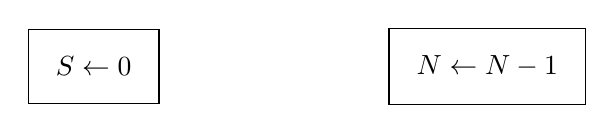
\begin{tikzpicture}
\node[instruct] (init) at (0,0) {$S\leftarrow 0$};
\node[instruct] (moins) at (5,0) {$N\leftarrow N-1$};
\end{tikzpicture}
\end{center}

\subsubsection{  
 علامت ورودی گرفتن و چاپ در خروجی ، متوازی الاضلاع می باشد }

\begin{center}
\begin{tikzpicture}
\node[input] (lire) at (0,0) { بخوان را $X$ };
\node[output] (afficher) at (5,0) { کن چاپ را $X$ };
\end{tikzpicture}
\end{center}

\subsubsection{ علامت بررسی شرط ، لوزی می باشد}

\begin{center}
\begin{tikzpicture}
\node[test] (test) at (0,0) {$N>0$};
\draw[suite] (test) -- ($(test)+(2,0)$) node[near start,yshift=7pt]{بله};
\draw[suite] (test) -- ($(test)+(-2,0)$) node[near start,yshift=7pt]{خیر};
\end{tikzpicture}
\end{center}


\newpage
\subsection{مثالهایی از الگوریتم و فلوچارت}

\subsubsection{مثال}

فلوچارتی رسم کنید که دو عدد A و B را به عنوان ورودی گرفته و حاصل جمع آنها را چاپ کند .

\begin{center}
\begin{tikzpicture}
\node[debutfin] (debut) at (0,0) {شروع};
\node[input] (lire) at (0,-2) { بخوان را $B$ و $A$ };
\node[instruct] (init) at (0,-4) {$C \leftarrow A + B$};
\node[output] (afficher) at (0,-6) { کن چاپ را $C$ };
\node[debutfin] (fin) at (0,-8) {پایان};
%Placementdesflèches
\draw[suite] (debut) -- (lire);
\draw[suite] (lire) -- (init);
\draw[suite] (init) -- (afficher);
\draw[suite] (afficher) -- (fin);
\end{tikzpicture}
\end{center}


\newpage
\subsubsection{مثال}

فلوچارتی رسم کنید که دو عدد را خوانده و حاصلضرب آنها را نمایش دهد 

\begin{center}
\begin{tikzpicture}
\node[debutfin] (debut) at (0,0) {شروع};
\node[input] (lire) at (0,-2) { بخوان را $B$ و $A$ };
\node[instruct] (init) at (0,-4) {$C \leftarrow A \times B$};
\node[output] (afficher) at (0,-6) { کن چاپ را $C$ };
\node[debutfin] (fin) at (0,-8) {پایان};
%Placementdesflèches
\draw[suite] (debut) -- (lire);
\draw[suite] (lire) -- (init);
\draw[suite] (init) -- (afficher);
\draw[suite] (afficher) -- (fin);
\end{tikzpicture}
\end{center}



\newpage
\subsubsection{مثال}

فلوچارتی رسم کنید که شعاع یک دایره را خوانده و مساحت و محیط آن را نمایش دهد .

\begin{center}
\begin{tikzpicture}
\node[debutfin] (debut) at (0,0) {شروع};
\node[input] (lire) at (0,-2) { بخوان را $r$ };
\node[instruct] (init) at (0,-4) {$A \leftarrow \pi \times r \times r$};
\node[instruct] (init2) at (0,-6) {$P \leftarrow 2 \times \pi \times r $};
\node[output] (afficher) at (0,-8) { کن چاپ را $A$ و $P$ };
\node[debutfin] (fin) at (0,-10) {پایان};
%Placementdesflèches
\draw[suite] (debut) -- (lire);
\draw[suite] (lire) -- (init);
\draw[suite] (init) -- (init2);
\draw[suite] (init2) -- (afficher);
\draw[suite] (afficher) -- (fin);
\end{tikzpicture}
\end{center}


\newpage
\subsubsection{مثال}

فلوچارتی رسم کنید که دو عدد را خوانده و سپس مقادیر آن دو عدد را با هم جا به جا کند .

\begin{center}
\begin{tikzpicture}
\node[debutfin] (a) at (0,0) {شروع};
\node[input] (b) at (0,-2) { بخوان را $B$ و $A$ };
\node[instruct] (c) at (0,-4) {$T \leftarrow A$};
\node[instruct] (d) at (0,-6) {$A \leftarrow B$};
\node[instruct] (e) at (0,-8) {$B \leftarrow T$};
\node[output] (f) at (0,-10) { کن چاپ را $A$ و $B$ };
\node[debutfin] (g) at (0,-12) {پایان};
%Placementdesflèches
\draw[suite] (a) -- (b);
\draw[suite] (b) -- (c);
\draw[suite] (c) -- (d);
\draw[suite] (d) -- (e);
\draw[suite] (e) -- (f);
\draw[suite] (f) -- (g);
\end{tikzpicture}
\end{center}


\newpage
\subsubsection{مثال}

فلوچارتی رسم کنید که یک عدد را دریافت کند و مشخص کند که عدد زوج است یا فرد 

\begin{itemize}
	\item یک عدد زوج است وقتی باقی مانده ی تقسیم آن عدد بر 2 برابر صفر باشد
	\item یک عدد فرد است وقتی باقی مانده ی تقسیم آن عدد بر 2 برابر با صفر نباشد
\end{itemize}

\begin{center}
\begin{tikzpicture}
\node[debutfin] (a) at (0,0) {شروع};
\node[input] (b) at (0,-2) { بخوان را $X$ };
\node[instruct] (c) at (0,-4) {$D \leftarrow X / 2$};
\node[instruct] (d) at (0,-6) {$R \leftarrow X - 2 \times D$};
\node[test] (test) at (0,-8) {$R = 0$};
\node[instruct] (e) at (2,-10) {است زوج $X$};
\node[instruct] (f) at (-2,-10) {است فرد $X$};
\node[debutfin] (g) at (0,-13) {پایان};
%Placementdesflèches
\draw[suite] (a) -- (b);
\draw[suite] (b) -- (c);
\draw[suite] (c) -- (d);
\draw[suite] (d) -- (test);
\draw[suite] (test) -| (e) node[near start,yshift=7pt]{بله};
\draw[suite] (test) -| (f) node[near start,yshift=7pt]{خیر};
\draw[suite] (e) |- (0,-11.5) -- (g);
\draw[suite] (f) |- (0,-11.5) -- (g);
\end{tikzpicture}
\end{center}



\newpage
\subsubsection{مثال}


فلوچارتی رسم کنید که عملکرد قدر مطلق را انجام دهد 

$$
|x| = \begin{cases}
x \geq 0 \qquad x \\
x < 0 \qquad -x 
\end{cases}
$$


\begin{center}
\begin{tikzpicture}
\node[debutfin] (a) at (0,0) {شروع};
\node[input] (b) at (0,-2) { بخوان را $X$ };
\node[test] (test) at (0,-4) {$X \geq 0$};
\node[instruct] (e) at (-2,-6) {$X \leftarrow -1 \times X$};
\node[output] (f) at (0,-9) { کن چاپ را $X$ };
\node[debutfin] (g) at (0,-11) {پایان};
%Placementdesflèches
\draw[suite] (a) -- (b);
\draw[suite] (b) -- (test);
\draw[suite] (test) -| (2,-6) node[near start,yshift=7pt]{بله} |- (0,-7.5) -- (f);
\draw[suite] (test) -| (e) node[near start,yshift=7pt]{خیر};
%\draw[suite] (d) |- (0,-7.5) -- (f);
\draw[suite] (e) |- (0,-7.5) -- (f);
\draw[suite] (f) -- (g);
\end{tikzpicture}
\end{center}



\newpage
\subsubsection{مثال}

فلوچارتی رسم کنید که عدد X را از ورودی بخواند و 
\begin{itemize}
	\item اگر X مثبت بود ، آن را در 2 ضرب کند و چاپ نماید
	\item اگر X منفی بود قدر مطلق X را چاپ کند 
\end{itemize}


\begin{center}
\begin{tikzpicture}
\node[debutfin] (a) at (0,0) {شروع};
\node[input] (b) at (0,-2) { بخوان را $X$ };
\node[test] (test) at (0,-4) {$X \geq 0$};
\node[instruct] (d) at (2,-6) {$X \leftarrow 2 \times X$};
\node[instruct] (e) at (-2,-6) {$X \leftarrow -1 \times X$};
\node[output] (f) at (0,-9) { کن چاپ را $X$ };
\node[debutfin] (g) at (0,-12) {پایان};
%Placementdesflèches
\draw[suite] (a) -- (b);
\draw[suite] (b) -- (test);
\draw[suite] (test) -| (d) node[near start,yshift=7pt]{بله};
\draw[suite] (test) -| (e) node[near start,yshift=7pt]{خیر};
\draw[suite] (d) |- (0,-7.5) -- (f);
\draw[suite] (e) |- (0,-7.5) -- (f);
\draw[suite] (f) -- (g);
\end{tikzpicture}
\end{center}


\newpage
\subsubsection{مثال}

فلوچارتی رسم کنید که عدد N را دریافت کند و N جمله ی اول دنباله ی 
$$
1 , 2 , 4 , 7 , 11 , 16 , \dots
$$

را چاپ کند 


\begin{center}
\begin{tikzpicture}
\node[debutfin] (a) at (0,0) {شروع};
\node[instruct] (b) at (0,-2) {$S \leftarrow 1 , C \leftarrow 1$};
\node[input] (c) at (0,-4) {بخوان را $N$};
\node[test] (test) at (0,-6) {$N > 0$};
\node[output] (d) at (3,-8) {کن چاپ را $S$};
\node[instruct] (f) at (3,-10) {$S \leftarrow S + C$};
\node[instruct] (g) at (3,-12) {$C \leftarrow C + 1$};
\node[instruct] (h) at (3,-14) {$N \leftarrow N - 1$};
\node[debutfin] (i) at (-3,-10) {پایان};
%Placementdesflèches
\draw[suite] (a) -- (b);
\draw[suite] (b) -- (c);
\draw[suite] (c) -- (test);
\draw[suite] (test) -| (d) node[near start,yshift=7pt]{بله};
\draw[suite] (test) -| (i) node[near start,yshift=7pt]{خیر};
\draw[suite] (d) -- (f);
\draw[suite] (f) -- (g);
\draw[suite] (g) -- (h);
\draw[suite] (h) -| (test);
\end{tikzpicture}
\end{center}


\newpage
\subsubsection{مثال}

فلوچارتی رسم کنید که عدد طبیعی N را از ورودی بخواند و مجموع و حاصل ضرب تعداد ارقام آن را محاسبه و چاپ نماید 




\begin{center}
\begin{tikzpicture}
\node[debutfin] (a) at (0,0) {شروع};
\node[instruct] (b) at (0,-2) {$S \leftarrow 0 , \ \leftarrow 1$};
\node[input] (c) at (0,-4) {بخوان را $N$};
\node[test] (test) at (0,-6) {$N > 0$};
\node[instruct] (d) at (3,-8) {$D \leftarrow N / 10$};
\node[instruct] (e) at (3,-10) {$R \leftarrow N - D \times 10$};
\node[instruct] (f) at (3,-12) {$P \leftarrow P \times R$};
\node[instruct] (g) at (3,-14) {$S \leftarrow S + R$};
\node[instruct] (h) at (3,-16) {$N \leftarrow D$};
\node[output] (i) at (-3,-8) {کن چاپ را $S$};
\node[output] (j) at (-3,-10) {کن چاپ را $P$};
\node[debutfin] (k) at (-3,-12) {پایان};
%Placementdesflèches
\draw[suite] (a) -- (b);
\draw[suite] (b) -- (c);
\draw[suite] (c) -- (test);
\draw[suite] (test) -| (d) node[near start,yshift=7pt]{بله};
\draw[suite] (test) -| (i) node[near start,yshift=7pt]{خیر};
\draw[suite] (d) -- (e);
\draw[suite] (e) -- (f);
\draw[suite] (f) -- (g);
\draw[suite] (g) -- (h);
\draw[suite] (h) -| (test);
\draw[suite] (i) -- (j);
\draw[suite] (j) -- (k);
\end{tikzpicture}
\end{center}



\newpage
\subsubsection{مثال}


فلوچارتی رسم کنید که دو عدد طبیعی M و N را از ورودی بخواند و حاصل ضرب آنها را از طریق جمع های متوالی به دست آورد 



\begin{center}
\begin{tikzpicture}
\node[debutfin] (a) at (0,0) {شروع};
\node[input] (b) at (0,-2) { بخوان را $N$ و $M$ };
\node[test] (test) at (0,-4) {$N > 0$};
\node[instruct] (c) at (3,-6) {$M \leftarrow M + M$};
\node[instruct] (d) at (3,-8) {$N \leftarrow N - 1$};
\node[output] (e) at (-3,-6) { کن چاپ را $M$ };
\node[debutfin] (f) at (-3,-8) {پایان};
%Placementdesflèches
\draw[suite] (a) -- (b);
\draw[suite] (b) -- (test);
\draw[suite] (test) -| (c) node[near start,yshift=7pt]{بله};
\draw[suite] (test) -| (e) node[near start,yshift=7pt]{خیر};
\draw[suite] (c) -- (d);
\draw[suite] (d) -| (test);
\draw[suite] (e) -- (f);
\end{tikzpicture}
\end{center}


\newpage
\subsubsection{مثال}

فلوچارتی رسم کنید که عدد صحیح و مثبت N را دریافت کند و باقی مانده و خارج قسمت تقسیم آن بر 2 را از طریق تفریق های متوالی به دست آورد 

\begin{center}
\begin{tikzpicture}
\node[debutfin] (a) at (0,0) {شروع};
\node[input] (b) at (0,-2) { بخوان را $N$ };
\node[instruct] (c) at (0,-4) {$C \leftarrow 0$};
\node[test] (test) at (0,-6) {$N > 2$};
\node[instruct] (d) at (3,-8) {$N \leftarrow N - 2$};
\node[instruct] (e) at (3,-10) {$C \leftarrow C + 1$};
\node[output] (f) at (-3,-8) { کن چاپ را $C$ };
\node[output] (g) at (-3,-10) { کن چاپ را $N$ };
\node[debutfin] (h) at (-3,-12) {پایان};
%Placementdesflèches
\draw[suite] (a) -- (b);
\draw[suite] (b) -- (c);
\draw[suite] (c) -- (test);
\draw[suite] (test) -| (d) node[near start,yshift=7pt]{بله};
\draw[suite] (test) -| (f) node[near start,yshift=7pt]{خیر};
\draw[suite] (d) -- (e);
\draw[suite] (e) -| (test);
\draw[suite] (f) -- (g);
\draw[suite] (g) -- (h);
\end{tikzpicture}
\end{center}



\newpage
\subsubsection{مثال}

فلوچارتی رسم کنید که یک عدد را از ورودی بخواند و فاکتوریل آن را محاسبه کند .

فاکتوریل عدد n را با 
$n!$
نشان می دهند و برابر است با :

$$
n! = n \times (n-1) \times (n-2) \times (n-3) \times \dots \times 1 
$$

\begin{center}
\begin{tikzpicture}
\node[debutfin] (a) at (0,0) {شروع};
\node[input] (b) at (0,-2) { بخوان را $N$ };
\node[instruct] (c) at (0,-4) {$fact \leftarrow 1$};
\node[test] (test) at (0,-6) {$N \geq 1$};
\node[instruct] (d) at (3,-8) {$fact \leftarrow fact \times N$};
\node[instruct] (e) at (3,-10) {$N \leftarrow N - 1$};
\node[output] (f) at (-3,-8) { کن چاپ را $fact$ };
\node[debutfin] (g) at (-3,-10) {پایان};
%Placementdesflèches
\draw[suite] (a) -- (b);
\draw[suite] (b) -- (c);
\draw[suite] (c) -- (test);
\draw[suite] (test) -| (d) node[near start,yshift=7pt]{بله};
\draw[suite] (test) -| (f) node[near start,yshift=7pt]{خیر};
\draw[suite] (d) -- (e);
\draw[suite] (e) -| (test);
\draw[suite] (f) -- (g);
\end{tikzpicture}
\end{center}



\newpage
\subsubsection{مثال}

فلوچارتی رسم کنید که مجموع اعداد 1 تا 100 را چاپ کند .


\begin{center}
\begin{tikzpicture}
\node[debutfin] (a) at (0,0) {شروع};
\node[instruct] (b) at (0,-2) {$I \leftarrow 100$};
\node[instruct] (c) at (0,-4) {$Sum \leftarrow 0$};
\node[test] (test) at (0,-6) {$I \geq 1$};
\node[instruct] (d) at (3,-8) {$Sum \leftarrow Sum + I$};
\node[instruct] (e) at (3,-10) {$I \leftarrow I - 1$};
\node[output] (f) at (-3,-8) { کن چاپ را $Sum$ };
\node[debutfin] (g) at (-3,-10) {پایان};
%Placementdesflèches
\draw[suite] (a) -- (b);
\draw[suite] (b) -- (c);
\draw[suite] (c) -- (test);
\draw[suite] (test) -| (d) node[near start,yshift=7pt]{بله};
\draw[suite] (test) -| (f) node[near start,yshift=7pt]{خیر};
\draw[suite] (d) -- (e);
\draw[suite] (e) -| (test);
\draw[suite] (f) -- (g);
\end{tikzpicture}
\end{center}



\newpage
\subsubsection{مثال}

فلوچارتی رسم کنید که تا زمانی که ورودی بزرگتر از صفر باشد 
از ورودی اعداد را دریافت کند و در انتها مجموع اعداد را نشان دهد


\begin{center}
\begin{tikzpicture}
\node[debutfin] (a) at (0,0) {شروع};
\node[input] (b) at (0,-2) {بخوان را $X$};
\node[instruct] (c) at (0,-4) {$Sum \leftarrow 0$};
\node[test] (test) at (0,-6) {$X > 0$};
\node[instruct] (d) at (3,-8) {$Sum \leftarrow Sum + X$};
\node[input] (e) at (3,-10) {بخوان را $X$};
\node[output] (f) at (-3,-8) { کن چاپ را $Sum$ };
\node[debutfin] (g) at (-3,-10) {پایان};
%Placementdesflèches
\draw[suite] (a) -- (b);
\draw[suite] (b) -- (c);
\draw[suite] (c) -- (test);
\draw[suite] (test) -| (d) node[near start,yshift=7pt]{بله};
\draw[suite] (test) -| (f) node[near start,yshift=7pt]{خیر};
\draw[suite] (d) -- (e);
\draw[suite] (e) -| (test);
\draw[suite] (f) -- (g);
\end{tikzpicture}
\end{center}



\newpage
\subsubsection{مثال}

فلوچارتی رسم کنید که 100 عدد را دریافت کند و بزرگترین آنها را نشان دهد 



\begin{center}
\begin{tikzpicture}
\node[debutfin] (a) at (0,0) {شروع};
\node[instruct] (b) at (0,-2) {$I \leftarrow 100$};
\node[input] (c) at (0,-4) {بخوان را $X$};
\node[instruct] (d) at (0,-6) {$MAX \leftarrow X$};
\node[test] (test) at (0,-8) {$I > 1$};
\node[input] (e) at (5,-10) {بخوان را $X$};
\node[test] (test2) at (5,-13) {$X > MAX$};
\node[instruct] (h) at (7,-15) {$MAX \leftarrow X$};
\node[instruct] (f) at (2,-16) {$I \leftarrow I - 1$};
\node[output] (i) at (-5,-12) {کن چاپ را $MAX$};
\node[debutfin] (j) at (-5,-14) {پایان};
%Placementdesflèches
\draw[suite] (a) -- (b);
\draw[suite] (b) -- (c);
\draw[suite] (c) -- (d);
\draw[suite] (d) -- (test);
\draw[suite] (test) -| (e) node[near start,yshift=7pt]{بله};
\draw[suite] (test) -| (i) node[near start,yshift=7pt]{خیر};
\draw[suite] (e) -- (test2);

\draw[suite] (test2) -| (h) node[near start,yshift=7pt]{بله};
\draw[suite] (test2) -| (f) node[near start,yshift=7pt]{خیر};

\draw[suite] (h) |- (f);
\draw[suite] (f) -| (test);


\draw[suite] (i) -- (j);
\end{tikzpicture}
\end{center}



\newpage
\subsubsection{مثال}

فلوچارتی رسم کنید که سه عدد را از ورودی دریافت کند و بزرگترین آنها را چاپ کند 



\begin{center}
\begin{tikzpicture}
\node[debutfin] (a) at (0,0) {شروع};
\node[input] (b) at (0,-2) {بخوان را $A$ و $B$ و $C$};
\node[test] (test) at (0,-4) {$A > B$};
\node[test] (test2) at (4,-10) {$B > C$};
\node[test] (test3) at (-3,-6) {$A > C$};
\node[output] (f1) at (-5,-8) { کن چاپ را $A$ };
\node[output] (f2) at (-1,-8) { کن چاپ را $C$ };
\node[output] (f3) at (2,-12) { کن چاپ را $B$ };
\node[output] (f4) at (6,-12) { کن چاپ را $C$ };
\node[debutfin] (g) at (0,-16) {پایان};
%Placementdesflèches
\draw[suite] (a) -- (b);
\draw[suite] (b) -- (test);

\draw[suite] (test) -| (test2) node[near start,yshift=8pt]{خیر};
\draw[suite] (test) -| (test3) node[near start,yshift=8pt]{بله};

\draw[suite] (test2) -| (f3) node[near start,yshift=8pt]{بله};
\draw[suite] (test2) -| (f4) node[near start,yshift=8pt]{خیر};


\draw[suite] (test3) -| (f1) node[near start,yshift=8pt]{بله};
\draw[suite] (test3) -| (f2) node[near start,yshift=8pt]{خیر};

\draw[suite] (f1) |- (0,-14) -- (g);
\draw[suite] (f2) |- (0,-14) -- (g);
\draw[suite] (f3) |- (0,-14) -- (g);
\draw[suite] (f4) |- (0,-14) -- (g);

\end{tikzpicture}
\end{center}







\subsubsection{مثال}

در مثال قبل برای اینکه دستور
\begin{tikzpicture}
\node[output] (a) at (0,0) { کن چاپ را $C$ };
\end{tikzpicture}
را دوبار به کار نبریم می توانیم فلوچارت را به صورت زیر بکشیم .


\begin{tikzpicture}
\node[debutfin] (a) at (0,0) {شروع};
\node[input] (b) at (0,-2) {بخوان را $A$ و $B$ و $C$};
\node[test] (test) at (0,-4) {$A > B$};
\node[test] (test2) at (4,-10) {$B > C$};
\node[test] (test3) at (-3,-6) {$A > C$};
\node[output] (f1) at (-5,-8) { کن چاپ را $A$ };
\node[output] (f2) at (0,-10) { کن چاپ را $C$ };
%\node[output] (f3) at (2,-12) { کن چاپ را $C$ };
\node[output] (f4) at (6,-12) { کن چاپ را $B$ };
\node[debutfin] (g) at (0,-16) {پایان};
%Placementdesflèches
\draw[suite] (a) -- (b);
\draw[suite] (b) -- (test);

\draw[suite] (test) -| (test2) node[near start,yshift=8pt]{خیر};
\draw[suite] (test) -| (test3) node[near start,yshift=8pt]{بله};

\draw[suite] (test2) -- (f2) node[near start,yshift=8pt]{خیر};
\draw[suite] (test2) -| (f4) node[near start,yshift=8pt]{بله};


\draw[suite] (test3) -| (f1) node[near start,yshift=8pt]{بله};
\draw[suite] (test3) -| (f2) node[near start,yshift=8pt]{خیر};

\draw[suite] (f1) |- (0,-14) -- (g);
\draw[suite] (f2) -- (0,-14) -- (g);
%\draw[suite] (f3) |- (0,-14) -- (g);
\draw[suite] (f4) |- (0,-14) -- (g);

%\draw[suite] (0,-9) -- (g);
\end{tikzpicture}





\newpage
\subsubsection{مثال}

همچنین می توانیم مثال قبل را به صورت کلی حل کنیم و مقدار شمارنده را 3 در نظر بگیریم

\begin{center}
\begin{tikzpicture}
\node[debutfin] (a) at (0,0) {شروع};
\node[instruct] (b) at (0,-2) {$I \leftarrow 3$};
\node[input] (c) at (0,-4) {بخوان را $X$};
\node[instruct] (d) at (0,-6) {$MAX \leftarrow X$};
\node[test] (test) at (0,-8) {$I > 1$};
\node[input] (e) at (5,-10) {بخوان را $X$};
\node[test] (test2) at (5,-13) {$X > MAX$};
\node[instruct] (h) at (7,-15) {$MAX \leftarrow X$};
\node[instruct] (f) at (2,-16) {$I \leftarrow I - 1$};
\node[output] (i) at (-5,-12) {کن چاپ را $MAX$};
\node[debutfin] (j) at (-5,-14) {پایان};
%Placementdesflèches
\draw[suite] (a) -- (b);
\draw[suite] (b) -- (c);
\draw[suite] (c) -- (d);
\draw[suite] (d) -- (test);
\draw[suite] (test) -| (e) node[near start,yshift=7pt]{بله};
\draw[suite] (test) -| (i) node[near start,yshift=7pt]{خیر};
\draw[suite] (e) -- (test2);

\draw[suite] (test2) -| (h) node[near start,yshift=7pt]{بله};
\draw[suite] (test2) -| (f) node[near start,yshift=7pt]{خیر};

\draw[suite] (h) |- (f);
\draw[suite] (f) -| (test);


\draw[suite] (i) -- (j);
\end{tikzpicture}
\end{center}


\newpage
\subsubsection{مثال}

فلوچارتی رسم کنید که اعداد فرد بین 1 تا 100 را چاپ کند


\begin{center}
\begin{tikzpicture}
\node[debutfin] (a) at (0,0) {شروع};
\node[instruct] (b) at (0,-2) {$I \leftarrow 1$};
\node[test] (test) at (0,-4) {$I \leq 100$};
\node[instruct] (c) at (3,-6) {$D \leftarrow I / 2$};
\node[instruct] (d) at (3,-8) {$R \leftarrow I - D \times 2$};
\node[test] (test2) at (3,-10) {$R \neq 0$};
\node[input] (f) at (6,-12) { کن چاپ را $I$ };
\node[instruct] (g) at (3,-14) {$I \leftarrow I + 1$};
\node[debutfin] (h) at (-3,-10) {پایان};
%Placementdesflèches
\draw[suite] (a) -- (b);
\draw[suite] (b) -- (test);
\draw[suite] (test) -| (c) node[near start,yshift=7pt]{بله};
\draw[suite] (test) -| (h) node[near start,yshift=7pt]{خیر};
\draw[suite] (c) -- (d);
\draw[suite] (d) -- (test2);
\draw[suite] (test2) -| (f) node[near start,yshift=8pt]{بله};
\draw[suite] (test2) -- (g) node[near start,xshift=-10pt]{خیر};
\draw[suite] (f) |- (g);
\draw[suite] (g) -| (test);
\end{tikzpicture}
\end{center}




\newpage
\subsubsection{مثال}


فلوچارتی رسم کنید که میانگین اعداد زوج بین 1 تا 100 را چاپ کند

\begin{center}
\begin{tikzpicture}
\node[debutfin] (a) at (0,0) {شروع};
\node[instruct] (b) at (0,-2) {$I \leftarrow 1 \:,\: Sum \leftarrow 0 \:,\: C \leftarrow 0$};
\node[test] (test) at (0,-4) {$I \leq 100$};
\node[instruct] (e) at (3,-6) {$D \leftarrow I / 2$};
\node[instruct] (f) at (3,-8) {$R \leftarrow I - D \times 2$};
\node[test] (test2) at (3,-10) {$R = 0$};
\node[instruct] (g) at (7,-12) {$Sum \leftarrow Sum + I$};
\node[instruct] (m) at (7,-14) {$C \leftarrow C + 1$};
\node[instruct] (k) at (3,-14) {$I \leftarrow I + 1$};
\node[instruct] (h) at (-3,-8) {$Avg \leftarrow Sum / C$};
\node[output] (i) at (-3,-10) { کن چاپ را $Avg$ };
\node[debutfin] (j) at (-3,-12) {پایان};
%Placementdesflèches
\draw[suite] (a) -- (b);
\draw[suite] (b) -- (test);
\draw[suite] (test) -| (e) node[near start,yshift=7pt]{بله};
\draw[suite] (test) -| (h) node[near start,yshift=7pt]{خیر};
\draw[suite] (e) -- (f);
\draw[suite] (f) -- (test2) ;
\draw[suite] (test2) -| (g) node[near start,yshift=8pt]{بله};
\draw[suite] (test2) -- (k) node[near start,xshift=-10pt]{خیر};
\draw[suite] (g) -- (m);
\draw[suite] (m) -- (k);
\draw[suite] (k) -| (test);
\draw[suite] (test) -| (h);
\draw[suite] (h) -- (i);
\draw[suite] (i) -- (j);
\end{tikzpicture}
\end{center}



\newpage
\subsubsection{مثال}

تبدیل از مبنای 2 به مبنای 10


\begin{center}
\begin{tikzpicture}
\node[debutfin] (a) at (0,0) {شروع};
\node[instruct] (b) at (0,-1.8) {$M \leftarrow 1 \:,\: S \leftarrow 0 \:,\: C \leftarrow 0$};
\node[input] (c) at (0,-3.5) {بخوان را $X$};
\node[test] (test) at (0,-5.5) {$X > 0$};
\node[instruct] (d) at (4,-8) {$D \leftarrow X / 10$};
\node[instruct] (e) at (4,-10) {$R \leftarrow X - 10 \times D$};
\node[instruct] (f) at (4,-12) {$I \leftarrow C$};
\node[test] (test3) at (4,-14) {$I > 0$};
\node[instruct] (g) at (7,-15) {$M \leftarrow 2 \times M$};
\node[instruct] (h) at (7,-16.5) {$I \leftarrow I - 1$};
\node[instruct] (ii) at (0,-8) {$X \leftarrow D$};
\node[instruct] (i) at (0,-9.5) {$M \leftarrow 1$};
\node[instruct] (j) at (0,-11) {$C \leftarrow C + 1$};
\node[instruct] (k) at (0,-12.5) {$S \leftarrow S + M$};
\node[instruct] (l) at (0,-14) {$M \leftarrow R \times M$};
\node[output] (m) at (-4,-8) {کن چاپ را $S$};
\node[debutfin] (n) at (-4,-11) {پایان};
%Drawing Edges
\draw[suite] (a) -- (b);
\draw[suite] (b) -- (c);
\draw[suite] (c) -- (test);
\draw[suite] (test) -| (d) node[near start,yshift=7pt]{بله};
\draw[suite] (test) -| (m) node[near start,yshift=7pt]{خیر};
\draw[suite] (d) -- (e);
\draw[suite] (e) -- (f) ;
\draw[suite] (f) -- (test3);
\draw[suite] (test3) -| (g) node[near start,yshift=8pt]{بله};
\draw[suite] (test3) -- (l) node[near start,yshift=-10pt]{خیر};
\draw[suite] (g) -- (h);
\draw[suite] (h) -| (test3);
\draw[suite] (l) -- (k);
\draw[suite] (k) -- (j);
\draw[suite] (j) -- (i);
\draw[suite] (i) -- (ii);
\draw[suite] (ii) -- (test);
\draw[suite] (m) -- (n);
\end{tikzpicture}
\end{center}




\newpage
\subsubsection{مثال}

تبدیل از مبنای 2 به مبنای 10 ، به روشی بهینه تر ( چرا ؟ )


\begin{center}
\begin{tikzpicture}
\node[debutfin] (a) at (0,0) {شروع};
\node[instruct] (b) at (0,-1.8) {$M \leftarrow 1 \:,\: S \leftarrow 0 \:,\: C \leftarrow 0$};
\node[input] (c) at (0,-3.5) {بخوان را $X$};
\node[test] (test) at (0,-5.5) {$X > 0$};
\node[instruct] (d) at (4,-6.5) {$D \leftarrow X / 10$};
\node[instruct] (e) at (4,-8) {$R \leftarrow X - 10 \times D$};
\node[test] (test2) at (4,-10) {$R \neq 0$};
\node[instruct] (f) at (6,-12) {$I \leftarrow C$};
\node[test] (test3) at (6,-14) {$I > 0$};
\node[instruct] (g) at (9,-15) {$M \leftarrow 2 \times M$};
\node[instruct] (h) at (9,-16.5) {$I \leftarrow I - 1$};
\node[instruct] (ii) at (0,-8) {$X \leftarrow D$};
\node[instruct] (i) at (0,-9.5) {$M \leftarrow 1$};
\node[instruct] (j) at (0,-11) {$C \leftarrow C + 1$};
\node[instruct] (k) at (0,-12.5) {$S \leftarrow S + M$};
\node[instruct] (l) at (0,-14) {$M \leftarrow R \times M$};
\node[output] (m) at (-4,-8) {کن چاپ را $S$};
\node[debutfin] (n) at (-4,-11) {پایان};
%Drawing Edges
\draw[suite] (a) -- (b);
\draw[suite] (b) -- (c);
\draw[suite] (c) -- (test);
\draw[suite] (test) -| (d) node[near start,yshift=7pt]{بله};
\draw[suite] (test) -| (m) node[near start,yshift=7pt]{خیر};
\draw[suite] (d) -- (e);
\draw[suite] (e) -- (test2) ;
\draw[suite] (test2) -| (f) node[near start,yshift=8pt]{بله};
\draw[suite] (test2) |- (l) node[near start,xshift=-10pt]{خیر};
\draw[suite] (f) -- (test3);
\draw[suite] (test3) -| (g) node[near start,yshift=8pt]{بله};
\draw[suite] (test3) -- (l) node[near start,yshift=-10pt]{خیر};
\draw[suite] (g) -- (h);
\draw[suite] (h) -| (test3);
\draw[suite] (l) -- (k);
\draw[suite] (k) -- (j);
\draw[suite] (j) -- (i);
\draw[suite] (i) -- (ii);
\draw[suite] (ii) -- (test);
\draw[suite] (m) -- (n);
\end{tikzpicture}
\end{center}




\newpage
\subsubsection{مثال}

تبدیل از مبنای 10 به مبنای 2


\begin{center}
\begin{tikzpicture}
\node[debutfin] (a) at (0,0) {شروع};
\node[instruct] (b) at (0,-1.8) {$M \leftarrow 1 \:,\: S \leftarrow 0 \:,\: C \leftarrow 0$};
\node[input] (c) at (0,-3.5) {بخوان را $X$};
\node[test] (test) at (0,-5.5) {$X > 0$};
\node[instruct] (d) at (4,-8) {$D \leftarrow X / 2$};
\node[instruct] (e) at (4,-10) {$R \leftarrow X - 2 \times D$};
\node[instruct] (f) at (4,-12) {$I \leftarrow C$};
\node[test] (test3) at (4,-14) {$I > 0$};
\node[instruct] (g) at (7,-15) {$M \leftarrow 10 \times M$};
\node[instruct] (h) at (7,-16.5) {$I \leftarrow I - 1$};
\node[instruct] (ii) at (0,-8) {$X \leftarrow D$};
\node[instruct] (i) at (0,-10) {$M \leftarrow 1$};
\node[instruct] (j) at (0,-12) {$C \leftarrow C + 1$};
\node[instruct] (l) at (0,-14) {$S \leftarrow S + R \times M$};
\node[output] (m) at (-4,-8) {کن چاپ را $S$};
\node[debutfin] (n) at (-4,-11) {پایان};
%Drawing Edges
\draw[suite] (a) -- (b);
\draw[suite] (b) -- (c);
\draw[suite] (c) -- (test);
\draw[suite] (test) -| (d) node[near start,yshift=7pt]{بله};
\draw[suite] (test) -| (m) node[near start,yshift=7pt]{خیر};
\draw[suite] (d) -- (e);
\draw[suite] (e) -- (f) ;
\draw[suite] (f) -- (test3);
\draw[suite] (test3) -| (g) node[near start,yshift=8pt]{بله};
\draw[suite] (test3) -- (l) node[near start,yshift=-10pt]{خیر};
\draw[suite] (g) -- (h);
\draw[suite] (h) -| (test3);
\draw[suite] (l) -- (j);
\draw[suite] (j) -- (i);
\draw[suite] (i) -- (ii);
\draw[suite] (ii) -- (test);
\draw[suite] (m) -- (n);
\end{tikzpicture}
\end{center}


\newpage
\subsubsection{مثال}

فلوچارتی رسم کنید که یک عدد صحیح را دریافت کند و مقلوب آن را چاپ کند . مثال : مقلوب 425 می شود 524


\begin{center}
\begin{tikzpicture}
\node[debutfin] (a) at (0,0) {شروع};
\node[instruct] (b) at (0,-1.8) {$M \leftarrow 1 \:,\: S \leftarrow 0 \:,\: C \leftarrow 0$};
\node[input] (c) at (0,-3.5) {بخوان را $X$};
\node[test] (test) at (0,-5.5) {$X > 0$};
\node[instruct] (d) at (4,-8) {$D \leftarrow X / 10$};
\node[instruct] (e) at (4,-10) {$R \leftarrow X - 10 \times D$};
\node[instruct] (f) at (4,-12) {$I \leftarrow C$};
\node[test] (test3) at (4,-14) {$I > 0$};
\node[instruct] (g) at (7,-15) {$M \leftarrow 10 \times M$};
\node[instruct] (h) at (7,-16.5) {$I \leftarrow I - 1$};
\node[instruct] (ii) at (0,-8) {$X \leftarrow D$};
\node[instruct] (i) at (0,-10) {$M \leftarrow 1$};
\node[instruct] (j) at (0,-12) {$C \leftarrow C + 1$};
\node[instruct] (l) at (0,-14) {$S \leftarrow S + R \times M$};
\node[output] (m) at (-4,-8) {کن چاپ را $S$};
\node[debutfin] (n) at (-4,-11) {پایان};
%Drawing Edges
\draw[suite] (a) -- (b);
\draw[suite] (b) -- (c);
\draw[suite] (c) -- (test);
\draw[suite] (test) -| (d) node[near start,yshift=7pt]{بله};
\draw[suite] (test) -| (m) node[near start,yshift=7pt]{خیر};
\draw[suite] (d) -- (e);
\draw[suite] (e) -- (f) ;
\draw[suite] (f) -- (test3);
\draw[suite] (test3) -| (g) node[near start,yshift=8pt]{بله};
\draw[suite] (test3) -- (l) node[near start,yshift=-10pt]{خیر};
\draw[suite] (g) -- (h);
\draw[suite] (h) -| (test3);
\draw[suite] (l) -- (j);
\draw[suite] (j) -- (i);
\draw[suite] (i) -- (ii);
\draw[suite] (ii) -- (test);
\draw[suite] (m) -- (n);
\end{tikzpicture}
\end{center}




\newpage
\subsubsection{مثال}

فلوچارتی رسم کنید که عدد طبیعی و دلخواه X را دریافت نماید و مقسوم علیه های آن را چاپ کند 


\begin{center}
\begin{tikzpicture}
\node[debutfin] (a) at (0,0) {شروع};
\node[input] (b) at (0,-1.8) {بخوان را $X$};
\node[instruct] (c) at (0,-3.5) {$C \leftarrow X$};
\node[test] (test) at (0,-5.5) {$C > 0$};
\node[instruct] (d) at (4,-7) {$D \leftarrow X / C$};
\node[instruct] (e) at (4,-9) {$R \leftarrow X - C \times D$};
\node[test] (test2) at (4,-11) {$R = 0$};
\node[output] (h) at (4,-14.5) {کن چاپ را $S$};
\node[instruct] (i) at (0,-11) {$C \leftarrow C - 1$};
\node[debutfin] (j) at (-4,-11) {پایان};
%Drawing Edges
\draw[suite] (a) -- (b);
\draw[suite] (b) -- (c);
\draw[suite] (c) -- (test);
\draw[suite] (test) -| (d) node[near start,yshift=7pt]{بله};
\draw[suite] (test) -| (j) node[near start,yshift=7pt]{خیر};
\draw[suite] (d) -- (e);
\draw[suite] (e) -- (test2);
\draw[suite] (test2) -- (h) node[near start,xshift=10pt]{بله};
\draw[suite] (test2) -- (i) node[near start,yshift=-10pt]{خیر};
\draw[suite] (i) -- (test);
\draw[suite] (h) -| (i);
\end{tikzpicture}
\end{center}




\newpage
\subsubsection{مثال}

فلوچارتی رسم کنید که عدد طبیعی و دلخواه X را دریافت نماید و مقسوم علیه های زوج آن را چاپ کند 


\begin{center}
\begin{tikzpicture}
\node[debutfin] (a) at (0,0) {شروع};
\node[input] (b) at (0,-1.8) {بخوان را $X$};
\node[instruct] (c) at (0,-3.5) {$C \leftarrow X$};
\node[test] (test) at (0,-5.5) {$C > 0$};
\node[instruct] (d) at (4,-6.5) {$D \leftarrow X / C$};
\node[instruct] (e) at (4,-8) {$R \leftarrow X - C \times D$};
\node[test] (test2) at (4,-10) {$R = 0$};
\node[instruct] (f) at (7,-11) {$D \leftarrow C / 2$};
\node[instruct] (g) at (7,-12.5) {$R \leftarrow C - 2 \times D$};
\node[test] (test3) at (7,-14.5) {$R = 0$};
\node[output] (h) at (3,-14.5) {کن چاپ را $S$};
\node[instruct] (i) at (0,-10) {$C \leftarrow C - 1$};
\node[debutfin] (j) at (-4,-10) {پایان};
%Drawing Edges
\draw[suite] (a) -- (b);
\draw[suite] (b) -- (c);
\draw[suite] (c) -- (test);
\draw[suite] (test) -| (d) node[near start,yshift=7pt]{بله};
\draw[suite] (test) -| (j) node[near start,yshift=7pt]{خیر};
\draw[suite] (d) -- (e);
\draw[suite] (e) -- (test2);
\draw[suite] (test2) -| (f) node[near start,yshift=8pt]{بله};
\draw[suite] (test2) -- (i) node[near start,yshift=-10pt]{خیر};
\draw[suite] (f) -- (g);
\draw[suite] (g) -- (test3);
\draw[suite] (test3) -- (h) node[near start,yshift=10pt]{بله};
\draw[suite] (test3) -- ($(test3)+(0,-1.8)$) -| (i) node[near start,yshift=-10pt]{خیر};
\draw[suite] (i) -- (test);
\draw[suite] (h) -| (i);
\end{tikzpicture}
\end{center}


\newpage
\section{کامپیوتر چیست؟}

کامپیوتر ماشینی است که می تواند برای انجام عملیات محاسباتی و منطقی  به کار گرفته شود .

یک کامپیوتر کامل شامل : 
\begin{itemize}
	\item سخت افزار
	\item سیستم عامل 
	\item رابط های ورودی و خروجی
\end{itemize}

می باشد .

\section{سخت افزار چیست؟}

سخت افزار کامپیوتر شامل اجزای فیزیکی و قابل لمس کامپیوتر می باشد ، مثل :

\begin{latin}
\begin{itemize}
	\item CPU (Central Processing Unit)
	\item Motherboard
	\item Hard Disk
	\item Monitor
	\item Keyboard
\end{itemize}
\end{latin}

\section{اجزای سخت افزاری کامپیوتر}

\subsubsection{Case}

Case
کامپیوتر ، قطعات سیستم کامپیوتری را در خود نگه می دارد و از آنها در برابر برخورد خارجی محافظت می کند، همچنین ساز و کاری را برای چرخش هوا و خنک سازی قطعات فراهم می کند .

\subsubsection{منبع تغذیه \lr{(Power Supply)}}

منبع تغذیه ولتاژ AC برق شهری را به ولتاژ  DC با اندازه های متفاوت و مناسب برای استفاده ی قطعات کامپیوتر فراهم می کند ، همچنین منبع تغذیه رابط های مختلفی را برای تغذیه ی برق قطعات مختلف کامپیوتر دارا می باشد .

\subsubsection{ مادربورد \lr{(MotherBoard)}}

MotherBoard
قطعه ی اصلی سیستم کامپیوتری است و یک برد با مدار های مجتمع و درگاه هایی می باشد که قطعات مختلف کامپیوتر از جمله :

\begin{latin}
\begin{itemize}
	\item CPU
	\item Hard Disk
	\item RAM
	\item CD \& DVD Drive
\end{itemize}
\end{latin}


را به هم متصل می کند .

\subsubsection{CPU}

CPU
اکثر اعمال محاسباتی را انجام می دهد که عملکرد کامپیوتر را محقق می سازد و به عنوان مغز کامپیوتر شناخته می شود .

CPU
دستورالعمل های برنامه را برای اجرا از 
RAM
دریافت می کند 

\lr{clock speed}
یکی از مشخصه های 
CPU
می باشد که تعیین می کند دستورالعمل ها با چه سرعتی اجرا شوند و با واحد GHz بیان می شود .

CPU
های مدرن قابلیت Overclock را فراهم می کنند که باعث افزایش عملکرد CPU 
می شود ولی دمای
CPU
را افزایش می دهد و بنابراین به سیستم خنک سازی بهتری نیازمند است .

\subsubsection{RAM}

کد ها و داده هایی را که توسط CPU
در حال استفاده و دسترسی هستند در خود نگه می دارد .

\subsubsection{ROM}

BIOS
را در خود نگه می دارد که وقتی کامپیوتر روشن می شود اجرا می شود .

فرآیندی که هنگام روشن شدن کامپیوتر توسط 
BIOS
انجام می شود ، 
Bootstrapping
نام دارد .

\subsubsection{درگاه \lr{(BUS)}}

CPU
را به قسمت های مختلف داخلی کامپیوتر متصل می کند

\subsubsection{کارت گرافیک \lr{(Video Card)}}

محاسبات گرافیکی کامپیوتر را انجام می دهد 


\section{نرم افزار چیست؟}

نرم افزار مجموعه ای از اطلاعات و دستوراالعمل هایی است که می تواند توسط سخت افزار ذخیره و اجرا شود و تعیین می کند که کامپیوتر چه کاری را انجام دهد .


\subsection{انواع گروه بندی نرم افزار}

\begin{itemize}
	\item نرم افزارهای سیستمی
	\item نرم افزارهای زمان حقیقی
	\item نرم افزارهای تجاری
	\item نرم افزار های مهندسی و علمی
	\item نرم افزار های تعبیه شده
	\item نرم افزار های کامپیوترهای شخصی
	\item نرم افزارهای مبتنی بر وب
	\item نرم افزارهای هوش مصنوعی
\end{itemize}


\subsubsection{نرم افزارهای سیستمی}
مجموعه ای از برنامه هاست که برای سرویس دهی به برنامه های دیگر نوشته شده اند .

 مثل : 
\begin{itemize}
	\item کامپایلر ها
	\item ویراستار ها
	\item برنامه های مدیریت فایل
\end{itemize}


\subsubsection{مشخصه های نرم افزار های سیستمی}

\begin{itemize}
	\item بر هم کنش سنگین با سخت افزار کامپیوتر
	\item استفاده سنگین توسط چند کاربر
	\item لزوم زمان بندی برای انجام کارها
	\item مدیریت فرآیند و اشتراک منابع
	\item ساختمان داده های پیچیده
	\item واسطهای خارجی چندگانه
\end{itemize}



\subsubsection{نرم افزارهای زمان حقیقی}

نرم افزاری که رویداد های جهان واقعی را همانطوری که رخ می دهند، نظارت ، تحلیل و کنترل می کنند .

\subsubsection{عناصر نرم افزار زمان حقیقی}

\begin{itemize}
	\item قطعه جمع آوری کننده داده ها
	\begin{itemize}
		\item اطلاعات را از محیط خارجی جمع آوری و قالب بندی می کند .
	\end{itemize}
	\item قطعه تحلیل کننده
	\begin{itemize}
		\item اطلاعات را بنا به نیاز کاربردی انتقال می دهد .
	\end{itemize}
	\item قطعه کنترل / خروجی
	\begin{itemize}
		\item به محیط خارجی پاسخ می دهد
	\end{itemize}
	\item قطعه نظارت
	\begin{itemize}
		\item همه ی قطعات دیگر را هماهنگ می کند .
	\end{itemize}
\end{itemize}



\subsubsection{نرم افزار های تجاری}
این نوع برنامه های کاربردی، داده های موجود را دوباره به شیوه ای سازماندهی می کند که عملیات تجاری و تصمیم گیری مدیریتی تسهیل شوند .


\subsubsection{نرم افزارهای تعبیه شده}
برای کنترل محصولات و سیستم های مربوط به بازارهای صنعتی و مصرفی به کار می رود .

مثل : 

\begin{itemize}
	\item صفحه کلید برای ماکروویو
	\item عملیات دیجیتال در خودرو
	\begin{itemize}
		\item کنترل سوخت
		\item صفحه نمایش داشبورد
		\item سیستم ترمز
	\end{itemize}
\end{itemize}


\section{سیستم عامل چیست؟}

سیستم عامل برنامه ای است که سخت افزار کامپیوتر را مدیریت می کند ، همچنین سیستم عامل به عنوان یک رابط بین کاربر و سخت افزار کامپیوتر می باشد 

\subsection{نمونه هایی از سیستم عامل های کامپیوترهای شخصی}

\begin{latin}
\begin{itemize}
	\item Microsoft Windows
		\begin{itemize}
			\item Windows NT - 1993
			\item Windows 98 - 1998 
			\item Windows Me - 2000
			\item Windows XP - 2001 
			\item Windows Vista - 2007
			\item Windows 7 - 2009 
			\item Windows 8 - 2012 
			\item Windows 10 - 2015 
		\end{itemize}
	\item MacOS
		\begin{itemize}
			\item Mac OS X Kodiak - 2000
			\item Mac OS X 10.2 Jaguar - 2002
			\item Mac OS X Panther - 2003
			\item Mac OS X Tiger -  2005
			\item Mac OS X Leopard - 2007
			\item Mac OS X Snow Leopard - 2009
			\item Mac OS X Lion - 2011
			\item OS X Mountain Lion - 2012
			\item OS X Mavericks - 2013
			\item OS X Yosemite - 2014
			\item OS X El Capitan - 2015
			\item macOS Sierra - 2016
			\item macOS High Sierra - 2017
			\item macOS Mojave - 2018
			\item macOS Catalina - 2019
		\end{itemize}
	\item Linux
		\begin{itemize}
			\item Debian
			\begin{itemize}
				\item Linux Mint 
				\item Ubuntu
			\end{itemize}
			\item Fedora
			\begin{itemize}
				\item Red Hat
			\end{itemize}
		\end{itemize}
\end{itemize}
\end{latin}

\subsection{نمونه هایی از سیستم عامل های تلفن های همراه}

\begin{latin}
\begin{itemize}
	\item Android
	\begin{itemize}
		\item Android 1.5 Cupcake (API 3) 
		\item Android 1.6 Donut (API 4) 
		\item Android 2.0 Eclair (API 5) 
		\item Android 2.3 Gingerbread (API 9) 
		\item Android 4.0 Ice Cream Sandwich (API 14) 
		\item Android 4.4 KitKat (API 19) 
		\item Android 5.0 Lollipop (API 21) 
		\item Android 6.0 Marshmallow (API 23) 
		\item Android 7.0 Nougat (API 24) 
		\item Android 8.0 Oreo (API 26) 
		\item Android 9 Pie (API 28) 
		\item Android 10 (API 29) 
	\end{itemize}
	\item iOS
	\item Windows Phone
\end{itemize}
\end{latin}

\section{برنامه نویسی چیست؟}

برنامه نویسی کامپیوتر فرآیند طراحی و ساخت یک برنامه ی اجرایی کامپیوتر است .

برنامه نویسی شامل موارد زیر می باشد :

\begin{itemize}
	\item آنالیز مسئله
	\item طراحی الگوریتم
	\item پیاده سازی الگوریتم
\end{itemize}

هدف برنامه نویسی تولید یک مجموعه از دستورالعمل ها برای خودکار سازی انجام یک وظیفه می باشد .

\subsection{انواع زبانهای برنامه نویسی}

انواع مختلفی از زبان های برنامه نویسی وجود دارد که هر کدام از آنها ویژگی ها و کاربرد های مختلفی دارند اما ساختار یکسانی دارند .

لزومی به دانستن همه ی زبان های برنامه نویسی نیست و درصورتی که شما یک زبان برنامه نویسی را خوب بدانید و چگونگی استفاده از متغیرها ، توابع ، کلاس ها و دیگر قابلیت های ارائه شده توسط یک زبان را بدانید در مدت زمان اندکی می توانید هر زبان برنامه نویسی دیگری را یاد بگیرید


\begin{latin}
\begin{itemize}
	\item C
	\item C++
	\item C\#
	\item Java
	\item Python
	\item PHP
	\item Javascript
	\item $\dots$
\end{itemize}
\end{latin}



\newpage
\chapter{شبکه و اینترنت}

\section{شبکه چیست؟}
. . . . . .
\subsection{انواع تکنولوژی در شبکه ها}
\subsubsection{تکنولوژی با سیم}
\subsubsection{تکنولوژی بی سیم}
. . . . . .
\section{انواع توپولوژی شبکه}
\subsubsection{Line}
\subsubsection{Bus}
\subsubsection{Star}
\subsubsection{Ring}
\subsubsection{Tree}
\subsubsection{Mesh}
\subsubsection{Fully-Connected}
. . . . . .
\section{سخت افزار های ایجاد شبکه}
\subsubsection{Hub}
\subsubsection{Switch}
\subsubsection{Router}
\subsubsection{Modem}
\subsubsection{Network-Interface-Card}
. . . . . .
\section{MAC-Address}
. . . . . .
\section{اینترنت چیست؟}
. . . . . .
\section{تاریخچه اینترنت}
. . . . . .
\section{IP Address}
. . . . . .
\section{ساختار IPv4}
. . . . . .
\section{انواع کلاسهای IP}
. . . . . .
\section{انواع پروتکل ها در شبکه}
. . . . . .
\subsection{DNS}
\subsection{ICMP}
\subsection{ARP}
\subsection{TCP}
\subsection{UDP}
\subsection{IPv6}


\newpage
\chapter{شبکه های اجتماعی}

\section{وبلاگ چیست؟}
. . . . . .
\subsection{انواع و نمونه هایی از وبلاگ ها}
. . . . . .
\section{تعریف شبکه اجتماعی}
. . . . . .
\subsection{انواع و نمونه هایی از شبکه های اجتماعی}
. . . . . .
\section{پیام رسان چیست؟}
. . . . . .
\subsection{انواع و نمونه هایی از پیام رسان ها}
. . . . . .
\section{فرق شبکه های اجتماعی و پیام رسان}
. . . . . .
\section{آثار شبکه های اجتماعی}
. . . . . .
\subsection{تاثیر شبکه های اجتماعی بر زندگی و اجتماع}
. . . . . .



\newpage
\chapter{امنیت}


\section{تعریف امنیت}
. . . . . .
\section{تعریف حمله}
. . . . . .
\subsection{انواع حمله ها}
. . . . . .
\subsection{نمونه هایی از حملات انجام شده}
. . . . . .
\section{ویروس ها}
. . . . . .
\subsection{روشهای مقابله با ویروس ها}
. . . . . .
\subsubsection{آنتی ویروس}
. . . . . .
\section{تروجان ها}
. . . . . .
\section{بد افزار چیست}
. . . . . .
\subsubsection{انواع بدافزار ها}
. . . . . .
\subsubsection{دیوار آتش}
. . . . . .


\end{document}